\documentclass[
  manuscript=article,  
  layout=preprint,  
]{format}

\usepackage{soul}
\usepackage{gensymb}

% --- blew is the area for authors ---

\usepackage[english]{babel}
\usepackage{comment}

% specify the .bib file for references
\addbibresource{reference.bib} 

% Make sure your article tile is within 12 words
\title{Uso de modelos de multinivel para incorporar la heterogeneidad en la evaluación de la susceptibilidad por movimientos en masa}

\author{Edier Aristizábal}
\affiliation{Departamento de Geociencias y Medio Ambiente, Universidad Nacional de Colombia, Medellín, Colombia}

% maximum five keywords
\keywords{landslide; susceptibility; logistic regression; spatial heterogeneity} 

\begin{document}

\begin{abstract}
Landslide susceptibility is defined as the likelihood of landslide occurrence under favorable terrain conditions. Traditional logistic regression models often fall short by assuming spatial homogeneity, ignoring the inherent variability of physical and environmental factors. To overcome this limitation, we used multilevel models that incorporate both fixed and random effects to capture variability among different spatial units. In this study, we employed a multilevel logistic regression model to assess landslide susceptibility in the Colombian Andes, incorporating both natural hydrological divisions and clustering-based spatial approaches.  This approach provides a more nuanced representation of susceptibility by addressing geographic heterogeneity. Two regionalization approaches were tested: natural basin divisions (Atrato, Cauca, Magdalena) and spatial clustering derived from morphometric characteristics. The results revealed that basin-based regionalization achieved a better model fit based on AIC and BIC metrics compared to the clustering-based model. This suggests that hydrological boundaries are more consistent in capturing landslides dynamics in our study area, likely due to their alignment with geomorphological processes. The fixed and random effect coefficients illustrated that variables such as elevation, relief, and area have significant variability depending on the regionalization method used. A major advantage of using multilevel models is their ability to incorporate spatial variability without artificially dividing the study area and training separate models for each subregion. By using shared information between different spatial units, these models can improve the estimation of both global and local effects.
\end{abstract}

\section{Introducción}
La susceptibilidad a movimientos en masa se define como la probabilidad de que ocurra un movimiento en masa en una área dada (\cite{corominas2014recommendations, brabb1984innovative, fell2008guidelines}). Esta probabilidad está vinculada con la condición natural del terreno, lo cual depende de diversos factores geológicos, hidrológicos, y geomorfológicos, entre otros (\cite{soeters1996, reichenbach2018}). A diferencia del concepto de amenaza, que incluye el componente temporal, la susceptibilidad se centra exclusivamente en las condiciones del terreno y su entorno que lo hacen favorable a la ocurrencia de movimientos en masa (\cite{corominas2014recommendations, fell2008guidelines}).

Para la evaluación de la susceptibilidad por movimientos en masa se han empleado tradicionalmente diversos enfoques, incluidos métodos basados en el conocimiento (heurísticos) (\cite{barredo2000comparing}), en datos (estadísticos) (\cite{korup2014landslide}) y con base física (\cite{montgomery1994}). Los modelos heurísticos se basan en observaciones previas y en la experiencia del analista, lo que los hace prácticos pero limitados en cuanto a reproducibilidad y objetividad (\cite{huang2020comparisons}). Los modelos con base física intentan representar los procesos físicos que conducen a la falla del terreno (\cite{sannino2024deterministic, palacio2020probabilistic}); sin embargo, su aplicación suele verse limitada por la disponibilidad de datos detallados y la intensidad del cálculo requerido (\cite{aristizabal2016shia_landslide, marin2021assessing}). Por otro lado, los modelos estadísticos se han popularizado debido a su capacidad para analizar grandes volúmenes de datos e identificar patrones que pueden predecir la ocurrencia de movimientos en masa (\cite{tehrani2022machine}). Estos modelos utilizan una variable respuesta, también denominada dependiente, que representa la ocurrencia de movimientos en masa, junto con un conjunto de variables predictoras, tambien denominadas como independientes, condicionantes o covariables, que describen las condiciones que favorecen su ocurrencia, como la pendiente, el tipo de suelo, el uso o cobertura del suelo, y la precipitación, entre otros.

En los últimos años, se ha observado un notable aumento en el uso de modelos estadísticos basados en aprendizaje automático (denominados \textit{machine learning}) para la evaluación de la susceptibilidad a movimientos en masa (\cite{tehrani2022machine}). Estos modelos han mejorado significativamente la capacidad de representar relaciones no lineales complejas entre las variables predictoras y la variable respuesta, logrando un excelente rendimiento en términos de predicción. Sin embargo, este incremento en la capacidad predictiva viene generalmente acompañado de una considerable pérdida en la interpretabilidad (\cite{youssef2023landslide}). Los modelos de aprendizaje automático, especialmente no-parametricos, como los basados en redes neuronales, se comportan como “cajas negras”, limitándose a proporcionar métricas de predicción sin aportar conocimiento sobre las causas subyacentes de los movimientos en masa (\cite{ermini2005artificial}). Esto representa una limitación para los usuarios, quienes necesitan comprender las interacciones entre los factores que contribuyen a la inestabilidad del terreno para poder tomar decisiones informadas.

Entre los modelos estadísticos tradicionales, la regresión logística se ha consolidado como uno de los enfoques más utilizados para la evaluación de la susceptibilidad a movimientos en masa (\cite{budimir2015systematic, reichenbach2018}). Este modelo establece una relación entre una variable respuesta binaria, que indica la presencia o ausencia de movimientos en masa, y un conjunto de variables predictoras categóricas o continuas que representan los factores condicionantes (\cite{ayalew2005application}). La regresión logística estima la probabilidad en cada unidad de mapeo de pertenecer a la clase movimiento en masa o no movimiento en masa del inventario utilizado, modelándola como un proceso de Bernoulli (\cite{ayalew2005application}). La relativa simplicidad de su interpretación y la facilidad para identificar el efecto de cada variable predictora han contribuido a su popularidad en el campo de la evaluación de amenazas naturales.

No obstante, una limitación significativa de la regresión logística y de otros modelos estadísticos convencionales, radica en la asignación de coeficientes constantes a las variables predictoras, asumiendo que la influencia de cada factor es homogénea en toda el área de estudio (\cite{anselin1996simple, cressie2015statistics}). Este supuesto de homogeneidad es problemático, ya que en la realidad las variables predictoras de los movimientos en masa son inherentemente heterogéneas y su influencia puede variar considerablemente a lo largo del espacio (\cite{petschko2012landslide}). Estudios previos han demostrado que la influencia de variables como la pendiente, la litología o el uso del suelo no es uniforme, sino que depende de las condiciones específicas de cada subregión del área de estudio (\cite{lombardo2020space}).

Para abordar esta heterogeneidad espacial, una de las estrategias más comunes en la evaluación de la susceptibilidad a movimientos en masa ha sido dividir el área de estudio en unidades homogéneas, como cuencas hidrográficas, y aplicar modelos separados en cada una de ellas. Esta estrategia es implementada por ejemplo por el Servicio Geológico Colombiano para los mapas de amenaza por movimientos en masa a nivel nacional (\cite{colombiano2013documento}). Aunque esta técnica permite tener en cuenta algunas diferencias espaciales, presenta también varias desventajas. En primer lugar, la división del área de estudio conlleva una disminución en la cantidad de datos disponibles para entrenar cada modelo, lo cual puede afectar la robustez de los resultados. Además, se incrementa significativamente la complejidad debido a la necesidad de entrenar y aplicar múltiples modelos independientes. Otro problema importante es la aparición de discontinuidades en los resultados obtenidos, ya que los modelos entrenados por separado tienden a generar diferencias en los bordes de las zonas modeladas, lo cual requiere ajustes y reprocesos.

Ante estas limitaciones, en las últimas décadas se han desarrollado modelos estadísticos espaciales que permiten incorporar la heterogeneidad de una manera más integral (\cite{anselin1988spatial, anselin2022spatial, lesage2009introduction, cressie2015statistics}). Entre estos modelos se encuentran los modelos jerárquicos o multiniveles (\cite{kumar2011hierarchical}), así como los modelos de regresión espacial ponderada (\cite{fotheringham2009geographically}). Los modelos multiniveles permiten la incorporación de variaciones en el intercepto o los coeficientes a lo largo del área de estudio, lo cual es ideal para capturar la heterogeneidad en las variables predictoras de los movimientos en masa. Estos modelos también permiten considerar distintos niveles de agrupación, como cuencas/subcuencas, ciudad/barrio, proporcionando una representación más detallada de la estructura espacial de los datos.

En este trabajo se presenta la aplicación de un modelo multinivel para la evaluación de la susceptibilidad por movimientos en masa a escala de subcrocuenca en los Andes colombianos, utilizando como grupos homogéneos las cuencas hidrográficas del Atrato, Cauca y Magdalena. El objetivo es presentar como los modelos multiniveles permiten una mejor representación de la heterogeneidad espacial, facilitando la incorporación de las variaciones en la influencia de las variables predictoras a lo largo del área de estudio. De esta manera, se espera contribuir al desarrollo de métodos más precisos y efectivos para la evaluación de la susceptibilidad por fenómenos geológicos, que puedan ser aplicados en Colombia.

\section{Modelo de Regresión Logística Multinivel}

Los modelos multiniveles, también conocidos como modelos jerárquicos, y en algunos casos mixtos o de regímenes espaciales, son un enfoque estadístico que permite la incorporación explícita de la estructura jerárquica o anidada de los datos (\cite{lee1996hierarchical}). Estos modelos combinan dos tipos de efectos: efectos fijos y efectos aleatorios. Los efectos fijos representan las relaciones generales entre las variables predictoras y la variable respuesta, aplicables a toda el área de estudio (\cite{kumar2011hierarchical}). Por otro lado, los efectos aleatorios permiten modelar la variabilidad que existe entre diferentes niveles jerárquicos, proporcionando estimaciones específicas para cada unidad espacial o región (\cite{kumar2011hierarchical}). Esta estructura es fundamental para capturar adecuadamente la heterogeneidad inherente a los datos espaciales cuando se tiene una organización natural en distintos niveles, donde las unidades de nivel inferior están agrupadas en unidades de nivel superior (\cite{wong1985hierarchical}). 

La formulación matemática de un modelo multinivel se basa en la combinación de efectos fijos y efectos aleatorios. Los efectos fijos se representan mediante coeficientes constantes que describen la relación promedio entre las variables predictoras y la variable respuesta. Por otro lado, los efectos aleatorios se modelan como términos adicionales que varían para cada grupo o unidad de nivel superior, permitiendo capturar la variabilidad específica entre estos grupos. Matemáticamente, un modelo multinivel se puede escribir como una combinación de ecuaciones que representan tanto la variabilidad global como la local (\cite{lee1996hierarchical}).

Consideremos una situación típica de dos niveles para una unidad de análisis en el nivel 1, $i$, que está anidada en la unidad de nivel 2, $j$. Supongamos que tenemos una variable dependiente de resultado binaria $Y_{ij}$ para el individuo (subcuenca) $i$ en el grupo (cuenca) $j$, que representa un inventario de movimientos en masa, donde $Y_{ij}$ toma el valor 1 si existe uno o mas movimientos en masa y 0 en caso contrario. Para este caso se puede utilizar un modelo de regresión logística con la función de enlace \textit{logit}, que representa el logaritmo de la relación entre la ocurrencia y no ocurrencia de un evento (\textit{odds}). Esta función transforma la relación lineal de las variables predictoras a una respuesta entre 0 y 1. De esta forma, la probabilidad $P(Y_{ij} = 1)$ se pueden expresar como:

\[
\text{logit}(P(Y_{ij} = 1)) = \log\left(\frac{P(Y_{ij} = 1)}{1 - P(Y_{ij} = 1)}\right) = \underbrace{\beta_{0j} + \sum_{j=1}^p\beta_{1j}X_{ij}}_\text{fectos fijos}+\underbrace{\sum_{l=1}^ru_{lj} + \varepsilon_i}_\text{efectos aleatorios}
\]

donde $\beta_{0j}$ y $\beta_{1j}$ son los coeficientes fijos que describen la relación entre la variable respuesta $Y$ y las variables predictoras \(X_{ij}\). Los coeficientes $\beta_{0j}$ y $\beta_{1j}$ se modelan a nivel de grupo. Podemos asumir que estos coeficientes siguen una distribución normal, de la siguiente forma:

\[
\beta_{0j} = \gamma_{00} + u_{0j}, \quad u_{0j} \sim \mathcal{N}(0, \sigma^2_{u0})
\]

\[
\beta_{1j} = \gamma_{10} + u_{1j}, \quad u_{1j} \sim \mathcal{N}(0, \sigma^2_{u1})
\]

donde $\gamma_{00}$ es el intercepto promedio entre todos los grupos.
$\gamma_{10}$ es el promedio del coeficiente del predictor $X_{ij}$ entre todos los grupos. $u_{0j}$ y $u_{1j}$ son los efectos aleatorios a nivel de grupo que capturan la variabilidad entre grupos para el intercepto y el coeficiente de $X_{ij}$, respectivamente. $\sigma^2_{u0}$ y $\sigma^2_{u1}$ representan la varianza de los efectos aleatorios del intercepto y del coeficiente, respectivamente.

Combinando los modelos de nivel individual y nivel grupal, el modelo completo se expresa como (\cite{lee1996hierarchical}):

\[
\text{logit}(P(Y_{ij} = 1)) = (\gamma_{00} + u_{0j}) + (\gamma_{10} + u_{1j}) X_{ij}
\]

o, de manera equivalente (\cite{wong1985hierarchical}):

\[
P(Y_{ij} = 1) = \frac{e^{(\gamma_{00} + u_{0j}) + (\gamma_{10} + u_{1j}) X_{ij}}}{1 + e^{(\gamma_{00} + u_{0j}) + (\gamma_{10} + u_{1j}) X_{ij}}}
\]

donde $P(Y_{ij} = 1)$ representa la probabilidad de que el resultado sea 1 para el individuo $i$ en el grupo $j$. $\sigma^2_{u0}$ representa la varianza del efecto aleatorio del intercepto a nivel de grupo. $\sigma^2_{u1}$ representa la varianza del efecto aleatorio del coeficiente del predictor $X_{ij}$ a nivel de grupo.

En este modelo de regresión logística multinivel, con coeficientes variables, el intercepto $\beta_{0j}$ varía entre grupos, lo que permite capturar diferencias en el nivel base del resultado para cada grupo. El coeficiente $\beta_{1j}$ del predictor $X_{ij}$ también varía entre grupos, lo que permite que el efecto o enfluencia del predictor cambie según el grupo. Los efectos aleatorios $u_{0j}$ y $u_{1j}$ permiten que tanto el intercepto como las pendientes cambien entre grupos, acomodando la heterogeneidad que no es capturada por los predictores a nivel individual.

En el contexto de la evaluación de la susceptibilidad a movimientos en masa, los modelos multiniveles resultan particularmente beneficiosos debido a la heterogeneidad espacial inherente, es decir, la variación en las características del terreno y las condiciones ambientales que pueden ocurrir de una ubicación a otra dentro del área de estudio. Se pueden definir niveles jerárquicos, como unidades de nivel inferior (por ejemplo, áreas más pequeñas como laderas o barrios) y unidades de nivel superior (como cuencas o municipios). En general, el nivel inferior se refiere a las unidades más pequeñas y detalladas, mientras que el nivel superior agrupa a estas unidades en categorías más amplias. Los efectos fijos permiten modelar cómo los factores (como pendiente, litología, uso del suelo) influyen de manera global en la susceptibilidad, mientras que los efectos aleatorios reflejan cómo estas relaciones pueden variar entre diferentes unidades espaciales, capturando mejor las diferencias locales. Por ejemplo, en algunas zonas, la pendiente puede tener una influencia predominante en la susceptibilidad a movimientos en masa debido a la presencia de suelos inestables, mientras que en otras, las condiciones climáticas específicas pueden favorecer el desarrollo de suelos con características distintas, afectando la susceptibilidad de manera diferenciada.

Dependiendo del contexto, se pueden utilizar dos o más niveles, pero se recomienda utilizar un número limitado (usualmente dos o tres niveles) para evitar complicaciones innecesarias en la modelización y garantizar resultados robustos (\cite{lee1996hierarchical, kumar2011hierarchical}).

Otra ventaja importante de los modelos multiniveles es la flexibilidad para incorporar información jerárquica sin necesidad de dividir el área de estudio de manera arbitraria y entrenar modelos independientes para cada subregión (\cite{lee1996hierarchical}). Esto evita los problemas de discontinuidad en los bordes de las zonas y permite utilizar la información compartida entre las distintas unidades para mejorar la estimación de los efectos globales y locales.

Sin embargo, los modelos multiniveles también presentan ciertas limitaciones. Una de las principales puede ser su mayor complejidad matemática y computacional, lo cual puede dificultar su implementación inicialmente. Además, la selección de la estructura adecuada del modelo (es decir, cuántos niveles incluir y cómo definir los efectos aleatorios) puede ser complicada y requiere conocer la dinámica espacial del fenómeno en estudio (\cite{kumar2011hierarchical}). Otro desafío es la interpretación de los efectos aleatorios, ya que estos pueden ser difíciles de comunicar a audiencias que no están familiarizadas con la estadística.

Existen diversos lenguajes de programación y paquetes que permiten trabajar con modelos multiniveles, cada uno con sus propias ventajas y desventajas. 

\textbf{R (lme4 y nlme)}: R es uno de los lenguajes más utilizados para la implementación de modelos multiniveles, principalmente a través de los paquetes lme4 y nlme. Estos paquetes permiten una gran flexibilidad para especificar efectos fijos y aleatorios, y ofrecen herramientas avanzadas para la visualización de resultados. Una ventaja importante de R es su comunidad amplia y activa, lo cual facilita el acceso a documentación y soporte. Sin embargo, la desventaja principal es que el procesamiento de grandes volúmenes de datos puede ser lento, lo que limita su uso en estudios de gran escala sin hardware especializado.

\textbf{Python (statsmodels y PyMC)}: En Python, los modelos multiniveles se pueden implementar utilizando statsmodels para enfoques más tradicionales, o PyMC para un enfoque bayesiano. PyMC es particularmente útil si se desea explorar la incertidumbre de los modelos mediante técnicas como Monte Carlo. Python es conocido por su versatilidad y su capacidad para integrarse con otros tipos de análisis y herramientas de aprendizaje automático de maquinas.

\textbf{Stan (a través de R o Python)}: Stan es un potente lenguaje para realizar inferencia bayesiana y es muy útil para modelos multiniveles complejos. Se puede acceder a través de interfaces en R (rstanarm) o Python (pystan). La principal ventaja de Stan es su precisión en la estimación de modelos complejos, y su capacidad para manejar estructuras jerárquicas detalladas. Sin embargo, su principal desventaja radica en la complejidad computacional y el tiempo necesario para realizar inferencias, especialmente cuando se aplican modelos con múltiples niveles y muchos parámetros.

\textbf{SPSS y Stata}: Para aquellos que prefieren interfaces gráficas, SPSS y Stata también ofrecen capacidades para trabajar con modelos multiniveles. Estas herramientas son más accesibles para usuarios con menos experiencia en programación, lo cual facilita la implementación de modelos sin necesidad de escribir código. La desventaja de estos programas es que son de pago y sus capacidades de personalización son más limitadas comparadas con las opciones de código abierto como R o Python.

La elección del lenguaje o software dependerá del propósito del estudio, las habilidades del investigador y la disponibilidad de recursos computacionales. Mientras que R y Python ofrecen opciones poderosas y flexibles para análisis detallados, herramientas como SPSS y Stata pueden ser más adecuadas para aquellos que buscan facilidad de uso en detrimento de la capacidad de personalización.

\section{Área de estudio y datos}

\par El área de estudio se encuentra al norte de 5$^{\circ}$N y abarca las Cordilleras Occidental y Central de los Andes colombianos, separadas por el cañón del Cauca. La región está delimitada por el río Atrato al oeste y el río Magdalena al este. Cubriendo aproximadamente 50,000 km$^2$, el área está dividida en 533 subcuencas dentro de las cuencas hidrográficas del Atrato (25\% de las cuencas), Cauca (50\%) y Magdalena (25\%). Aproximadamente el 73\% de estas cuencas tienen áreas menores de 100 km$^2$, con un área media de 48 km$^2$.

\par En este estudio se elaboró un catálogo de 13,777 deslizamientos superficiales y profundos que ocurrieron entre 1970 y 2023 (Fig.\ref{fig:localizacion}), detectados visualmente utilizando imágenes ópticas de alta resolución (\$<\$1\~m) en color real de Google Earth™.

\begin{figure}[ht!]
    \centering
      {\includegraphics[width=0.8\textwidth]{figures/localizacion.png}}
\caption{Mapa de localización del área de estudio en las Cordilleras Occidental y Central de los Andes colombianos. Los puntos rojos representan los movimientos en masa registrados entre 1970 y 2023. Se muestran los principales ríos y la delimitación de las cuencas del Atrato, Cauca y Magdalena.}
    \label{fig:localizacion}
\end{figure}

\par Inicialmente, se seleccionaron como variables predictoras para el área de estudio: área bajo la curva hipsométrica de la subcuenca, elevación media, pendiente media, relieve local medio, precipitación media anual, número de días con precipitación diaria acumulada \$>\$20\~mm, cobertura del suelo y geología predominante(\$G\$).

\par Los parámetros del terreno se calcularon utilizando el modelo digital de elevación (DEM) del radar de apertura sintética en banda L del satélite de observación terrestre Aaanzada (ALOS-PALSAR), con una resolución de píxel de 12.5\~m \cite{logan2014}.

\par Las métricas de precipitación se derivaron utilizando los datos de CHIRPS (\textit{Climate Hazard Group InfraRed Precipitation with Station Data}) \cite{funk2015}, versión 2.0, para datos de precipitación con una resolución de 5\~km desde 1981 hasta 2023. Para este cálculo se utilizó la plataforma Google Earth Engine (GEE) con lenguaje Javascript.

\par Se generó un mapa de cobertura del suelo utilizando datos del programa Copernicus Sentinel-2, con una resolución de 10\~m. Utilizando GEE, seleccionamos imágenes desde 2018 hasta 2023 con menos del 10\% de cobertura de nubes, eliminando efectos de sombra. El mapa se creó calculando el índice de vegetación de diferencia normalizada (NDVI) \cite{kriegler1969}, el índice de diferencia normalizada de construcciones (NDBI) \cite{zha2003}, el índice de diferencia normalizada de agua modificado (MNDWI) \cite{xu2006} y el índice de suelo desnudo (BSI) \cite{li2014}. La clasificación de cobertura del suelo se realizó con un algoritmo de bosque aleatorio (\textit{random forest}) del paquete Classifier de GEE \cite{breiman2001}.

\par Para implementar los modelos multiniveles, definimos regiones. En este estudio, utilizamos dos regiones distintas. El primer régimen corresponde a las divisiones naturales por las principales cuencas: Atrato, Cauca y Magdalena. El segundo régimen utilizó la clusterización aglomerativa basada en parámetros morfométricos y una matriz de conectividad espacial, aplicada con diferentes \$K\$ vecinos más cercanos para \$K\$ = 2, 3, 4, 5 y 6. La agrupación se implementó en Python utilizando la librería Scikit-Learn, guiada por el método del codo y el coeficiente de Silhouette \cite{scikit-learn2011}. El método del codo ayuda a identificar el número óptimo de grupos trazando la suma de cuadrados dentro del grupo contra $K$ para detectar el punto de inflexión \cite{thorndike1953}. El coeficiente de Silhouette (Sc) evalúa la cohesión dentro de los grupos y la separación entre los grupos, con un rango de \$-1\$ (mala agrupación) a \$+1\$ (agrupación fuerte) \cite{rousseeuw1987}.

\section{Resultados}

\subsection{Modelo de regresión logística}

\par Para seleccionar las variables predictoras a incorporar en los modelos se utilizó el Análisis de Componentes Principales (PCA) (Fig.~\ref{fig:PCA}). Los dos componentes principales obtenidos en el análisis PCA explicaron el 70\% de la varianza total. El análisis en la Figura \ref{fig:PCA} destaca cuatro grupos de predictores colineales: (i) elevación promedio de la subcuenca y pendiente promedio, (ii) área bajo la curva hipsometrica, elevación media, (iii) precipitación media anual, y (iv) área. A partir de estos resultados, se seleccionó de cada grupo un predictor: relieve, elevación, precipitación media anual y área. 

\begin{figure}[ht!]
    \centering
      {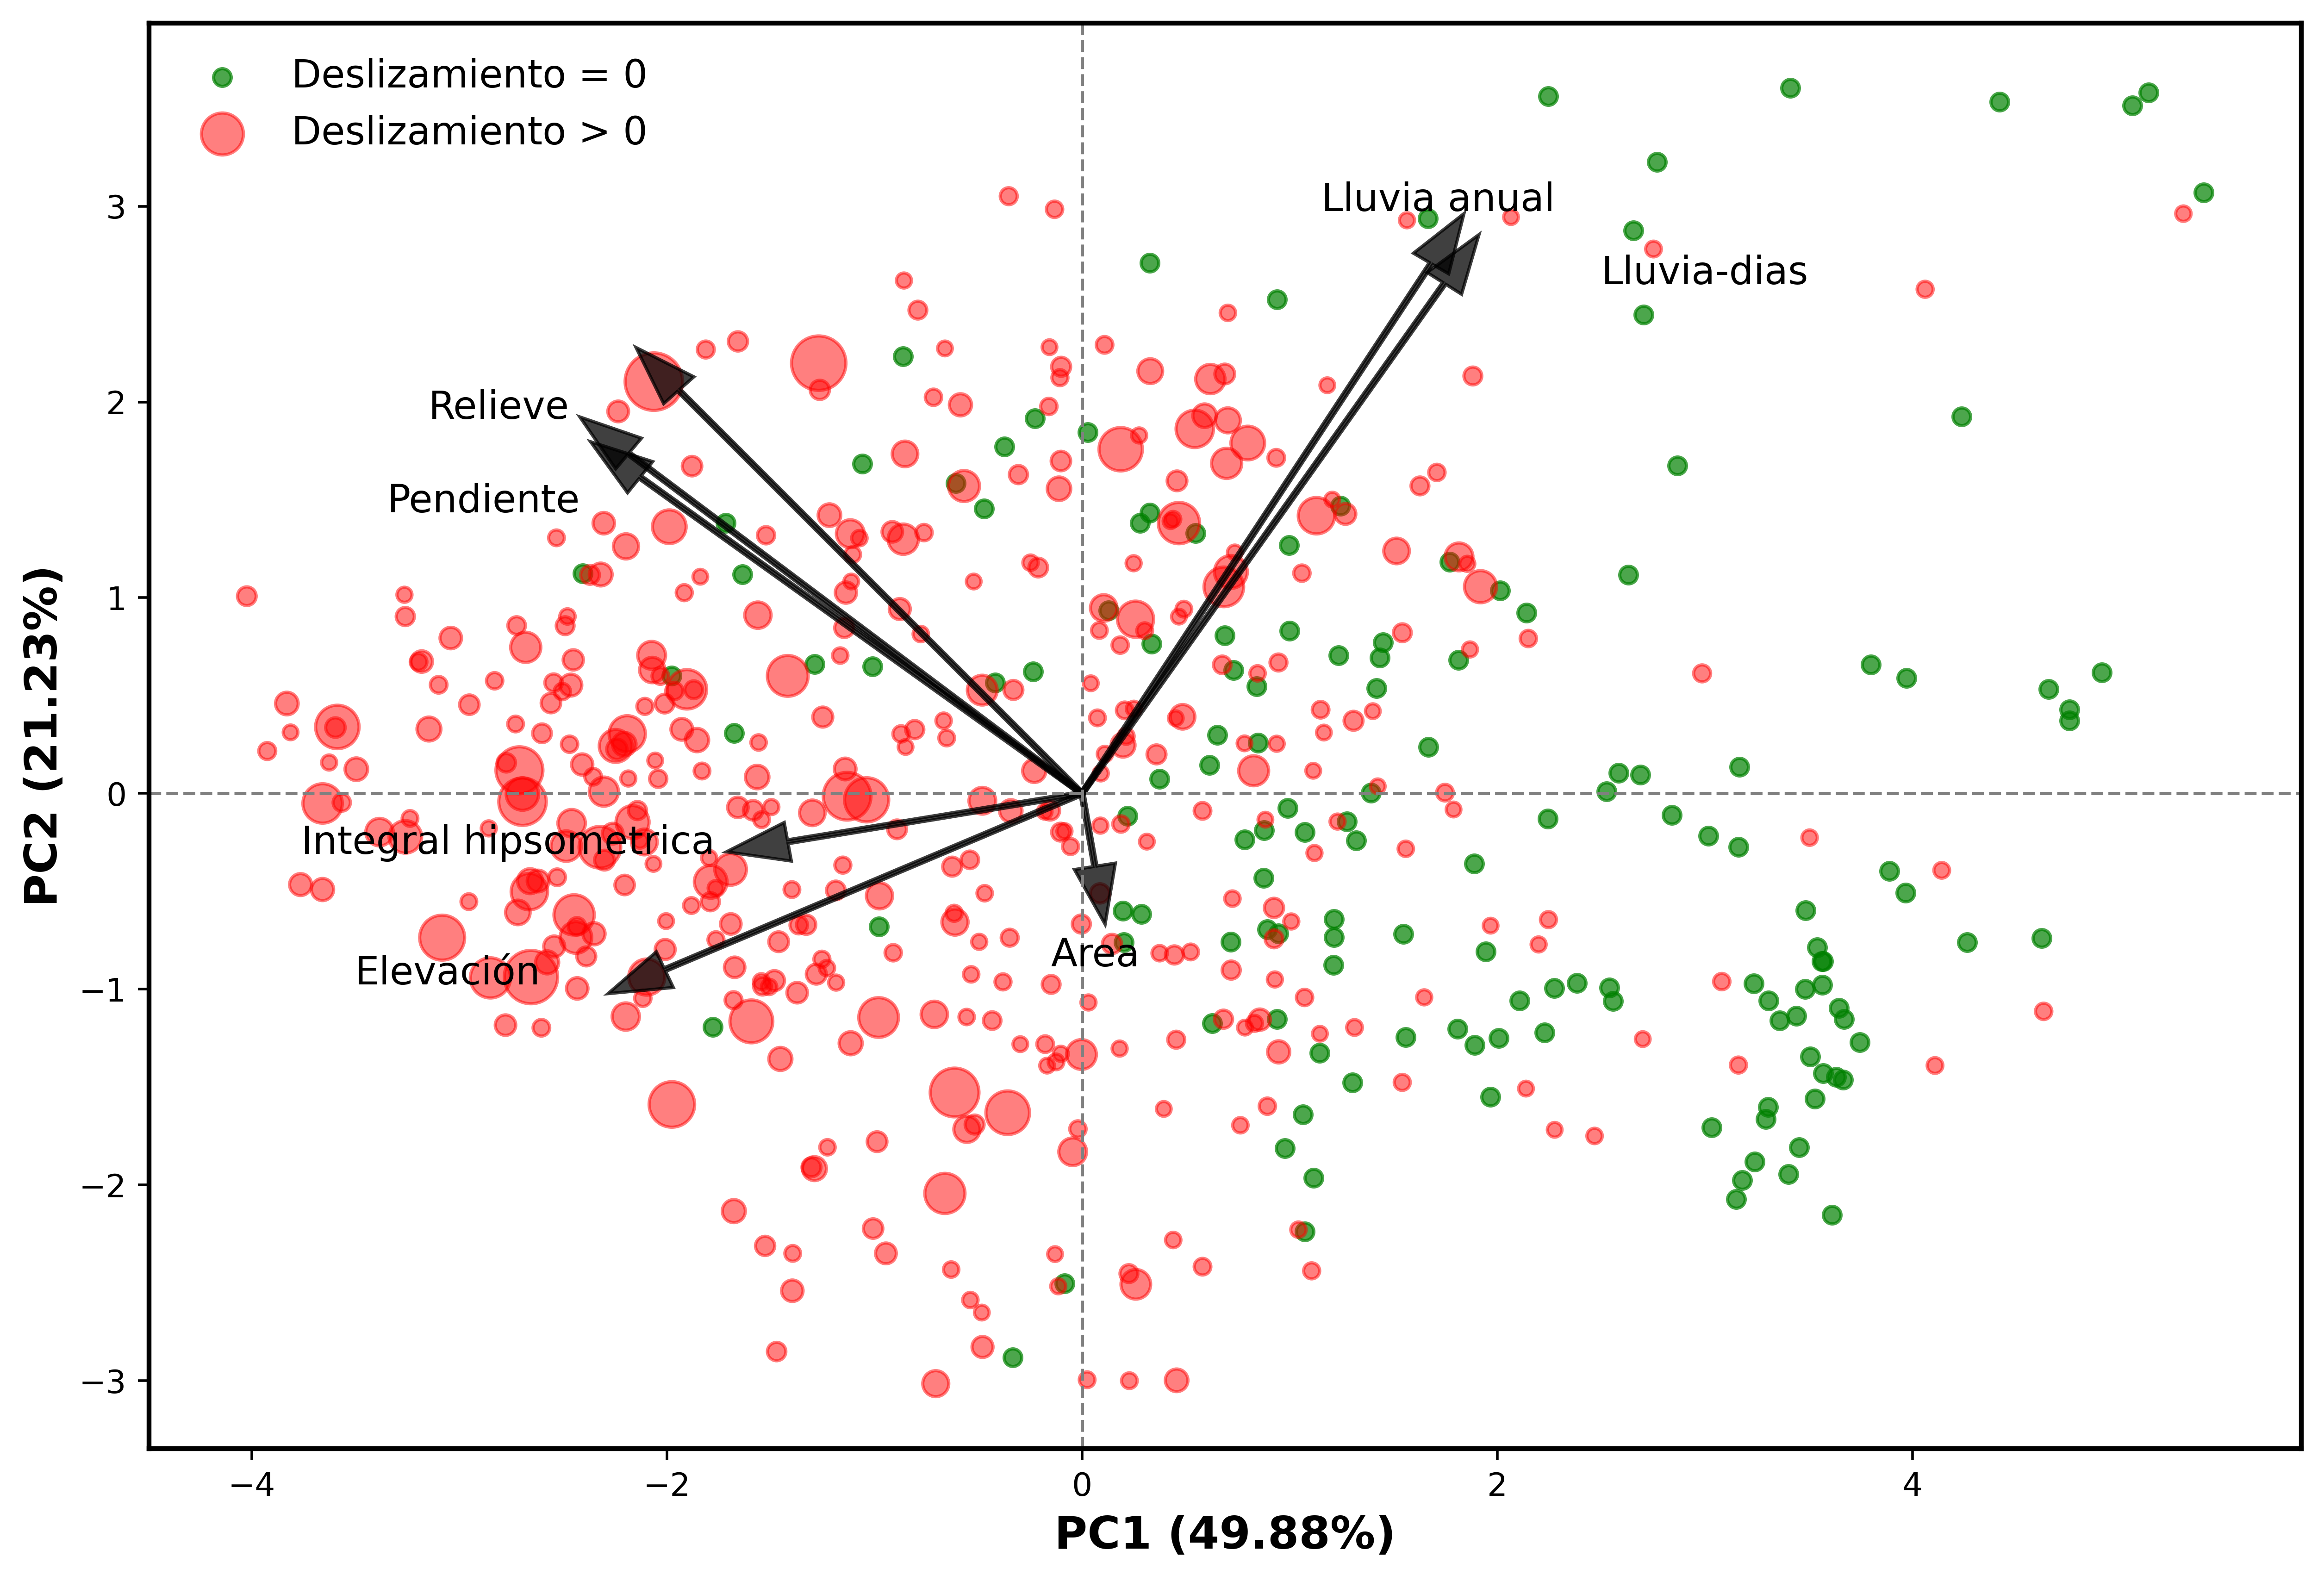
\includegraphics[width=1\textwidth]{figures/PCA.png}}
\caption{Análisis de Componentes Principales (PCA) para evaluar la relación entre las microcuencas con movimientos en masa y las variables predictoras. Se presentan los dos primeros componentes principales (PC1 y PC2), que explican el 49.9\% y el 21.2\% de la varianza total, respectivamente. Los puntos rojos indican microcuencas con presencia de movimientos en masa, mientras que los puntos verdes indican ausencia. Las flechas corresponden a las contribuciones de las variables predictoras}
    \label{fig:PCA}
\end{figure}

La Tabla \ref{tab:m1} presenta un resumen del modelo de regresión logística simple, con las estimaciones de los coeficientes para las variables predictoras seleccionadas. El intercepto tiene un coeficiente altamente significativo (valor P < 0.001). El valor Z indica cuán lejos está el coeficiente de ser cero en términos de desviaciones estándar, mientras que el valor de P nos dice cuán probable es obtener un valor de cero bajo la hipótesis nula. El coeficiente representa el logaritmo de la relación entre la ocurrencia y no ocurrencia de movimientos en masa cuando todas las variables predictoras son cero. 

Las variables predictoras, como la elevación, el relieve, el área y la lluvia anual, presentan coeficientes estadísticamente significativos, es decir valores por debajo de 0.05 (5\%). La variable de elevación tiene un coeficiente estimado que indica que existe una asociación positiva significativa entre la elevación y la probabilidad de ocurrencia de movimientos en masa. Esto sugiere que áreas con mayor elevación tienden a tener una mayor susceptibilidad a movimientos en masa. La variable de relieve indica que el relieve local es un predictor importante y positivo, aumentando la probabilidad de movimientos en masa en cuencas con mayor relieve. La variable del área también presenta un coeficiente significativo lo que representa que cuencas más grandes tienden a tener mas movimientos en masa. Por el contrario, la variable de lluvia anual tiene un coeficiente negativo, lo cual indica que existe una relación negativa entre la cantidad de precipitación anual y la ocurrencia de movimientos en masa. Esto podría sugerir que las áreas con precipitación mayor tienden a no presentar movimientos en masa, posiblemente debido a la adaptación del terreno o la vegetación.

Los estadísticos del modelo, en este caso el Cox \& Snell $R^2$ proporciona el ajuste del modelo. El valor obtenido indica un buen ajuste del modelo, aunque el valor específico debe interpretarse con cautela, ya que depende del contexto del estudio. Además, el criterio de información de Akaike (AIC) tiene un valor de 397.828, lo cual proporciona una medida del ajuste del modelo considerando su complejidad.

\begin{table}[!h]
\caption{Modelo de regresión logística multinivel}
\label{tab:m1}
\centering
\begin{tabular}[t]{ccccc}
\toprule
Variables & Estimate & Std\_Error & Z\_value & P\_value\\
\midrule
\cellcolor{gray!6}{(Intercepto)} & \cellcolor{gray!6}{1.762} & \cellcolor{gray!6}{0.173} & \cellcolor{gray!6}{10.164} & \cellcolor{gray!6}{< 0.001}\\
Elevación & 0.794 & 0.213 & 3.727 & < 0.001\\
\cellcolor{gray!6}{Relieve} & \cellcolor{gray!6}{1.242} & \cellcolor{gray!6}{0.214} & \cellcolor{gray!6}{5.802} & \cellcolor{gray!6}{< 0.001}\\
Área & 0.680 & 0.162 & 4.197 & < 0.001\\
\cellcolor{gray!6}{Lluvia anual} & \cellcolor{gray!6}{-0.508} & \cellcolor{gray!6}{0.173} & \cellcolor{gray!6}{-2.935} & \cellcolor{gray!6}{0.00333}\\
\midrule
Cox \& Snell $R^2$ & -308.745 & NA & NA & NA\\
\cellcolor{gray!6}{AIC} & \cellcolor{gray!6}{397.828} & \cellcolor{gray!6}{NA} & \cellcolor{gray!6}{NA} & \cellcolor{gray!6}{NA}\\
\bottomrule
\end{tabular}
\end{table}

\subsection{Modelos de regresión logística multiniveles}

\par Para implementar los modelos multiniveles es necesario establecer regiones homogéneas. La segmentación geográfica y natural en cuencas no necesariamente explica la ocurrencia de movimientos en masa. Aunque el área de estudio se divide naturalmente en las cuencas de los ríos Atrato, Cauca y Magdalena, utilizamos un análisis de agrupamiento espacial basado en parámetros morfométricos para identificar regiones homogéneas que pudieran explicar la ocurrencia de movimientos en masa (Fig.~\ref{fig:niveles}). Utilizamos clusterización aglomerativa espacial con diferentes números de vecinos. El mejor resultado, utilizando el método del codo y el índice de Silhouette, se obtuvo con $K=5$ vecinos y cuatro grupos (Fig.~\ref{fig:niveles}). El grupo A corresponde a los terrenos aluviales bajos a lo largo de las cuencas del Magdalena y Cauca; el grupo B representa los terrenos de alto relieve a lo largo del cañón del Cauca; el grupo C corresponde a los terrenos aluviales bajos a lo largo de la cuenca del Atrato, y el grupo D comprende las superficies de alta elevación y bajo relieve en el eje de la Cordillera Central.

La Figura \ref{fig:niveles} muestra los dos enfoques diferentes para definir las regiones espaciales multinivel utilizados en el análisis de susceptibilidad a movimientos en masa en el área de estudio. El mapa a la izquierda muestra la subdivisión del área de estudio basada en las principales cuencas hidrográficas: Atrato (verde), Cauca (rojo), y Magdalena (azul). Estas cuencas se utilizaron como unidades espaciales de nivel superior, capturando la heterogeneidad inherente a la variabilidad fisiográfica y ambiental de cada cuenca. El mapa a la derecha muestra el resultado de la clusterización espacial. Esta técnica permitió identificar agrupamientos que comparten características morfométricas similares, proporcionando una visión más detallada de las unidades espaciales en comparación con la división por cuencas hidrográficas.

\begin{figure}[ht!]
  \begin{minipage}{.48\linewidth}
    \centering
      {\includegraphics[width=1\textwidth]{figures/cuencas.png}}
  \end{minipage}\quad
  \begin{minipage}{.48\linewidth}
    \centering
      {\includegraphics[width=1\textwidth]{figures/cluster.png}}
  \end{minipage}
\caption{Comparación de los regímenes espaciales utilizados en el análisis multinivel de susceptibilidad a movimientos en masa. El mapa a la izquierda muestra la subdivisión en las principales cuencas hidrográficas (Atrato, Cauca y Magdalena). El mapa a la derecha muestra el resultado de la clusterización espacial utilizando $K$ vecinos más cercanos (KNN-5), dividiendo el área de estudio en cuatro grupos (A, B, C, D). Ambos enfoques buscan capturar la variabilidad espacial a diferentes escalas para mejorar la evaluación de la susceptibilidad.}
    \label{fig:niveles}
\end{figure}

La Figura \ref{fig:m2-table} presenta los resultados del modelo de regresión logística multinivel utilizando el paquete \textit{glmer} de R. El modelo especifica un intercepto aleatorio y pendientes aleatorias para cada uno de estos predictores agrupados por cuenca.  El Criterio de Información Bayesiano (BIC) también mide el ajuste, penalizando más fuertemente por la complejidad que el \textit{AIC}. El logaritmo de la verosimilitud (\textit{logLik}) mide qué tan bien el modelo se ajusta a los datos; valores más altos (menos negativos) indican un mejor ajuste. La \textit{desviación} es una medida del ajuste del modelo, similar a la suma de cuadrados residuales en modelos lineales. Valores más bajos son mejores. Los \textit{grados de libertad} residuales son básicamente el número de observaciones menos el número de parámetros estimados. Y los valores de \textit{Residuales} proporciona un resumen de las diferencias entre los valores observados y predichos. También se presentan los efectos aleatorios agrupados por cuenca en este caso. La varianza y desviación estándar muestran la variabilidad del intercepto y de las pendientes a lo largo de los diferentes grupos (cuenca). Para el intercepto la varianza es cero, lo que sugiere que no hay variación en el intercepto entre las cuencas. En cuanto a las variables predictoras la varianza y la desviación estándar indican cuánto varía su relación con el resultado en diferentes grupos (cuenca). Una varianza alta significa mayor variabilidad. La correlación entre efectos aleatorios como, una correlación de 0.85 entre el relieve medio de las cuencas y la elevación media, indica una relación positiva fuerte entre estas pendientes en las cuencas. \textit{NaN} indica que la correlación no está definida debido a una varianza cero en el efecto aleatorio correspondiente.

\begin{figure}[ht!]
    \label{fig:m2-table}
    \centering
      {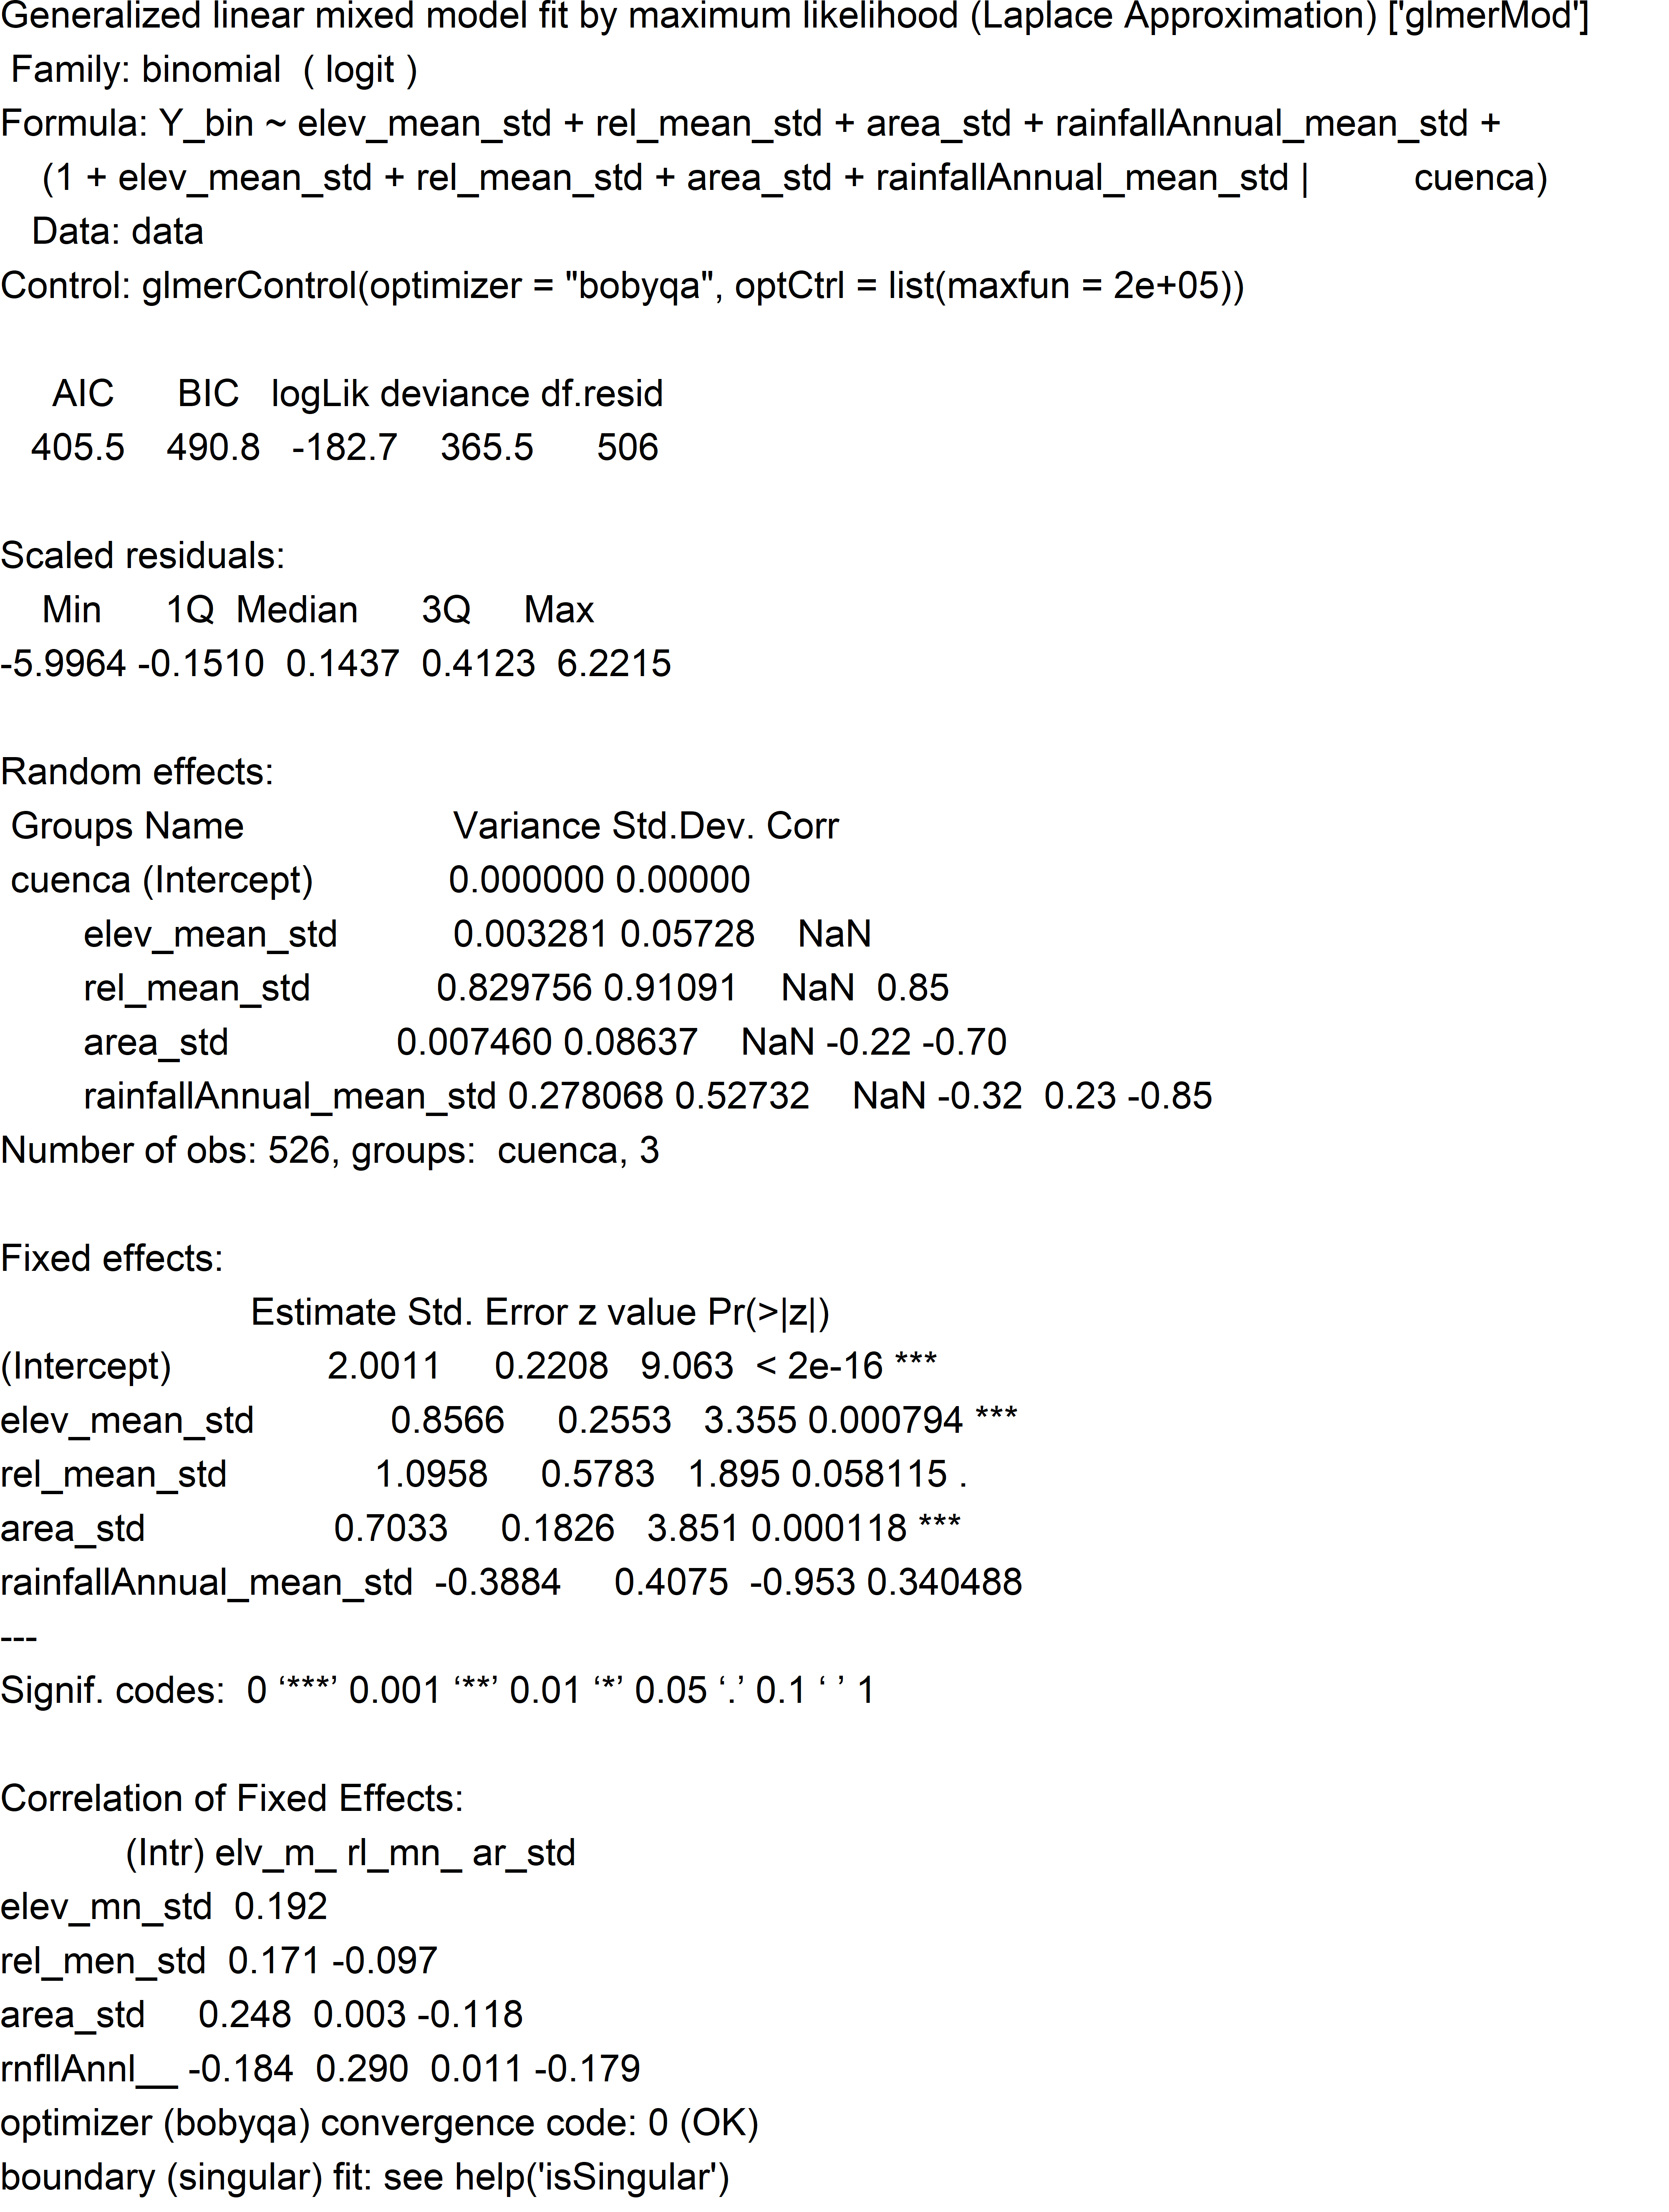
\includegraphics[width=0.6\textwidth]{figures/m2_summary.png}}
\caption{Resumen del modelo de regresión logística multinivel para la evaluación de la susceptibilidad a movimientos en masa, del paquete \textit{glmer} del lenguaje R.}
\end{figure}

En cuanto a los efectos fijos, los coeficientes representan el efecto promedio de cada variable predictora en todos los grupos. En cuanto a los coeficientes de las variables predictoras, por ejemplo elevación media de las cuencas, indican que un aumento de una unidad en la elevación, incrementa los logaritmos de las probabilidades de la ocurrencia de un movimiento en masa en 0.8566. La correlación de efectos fijos muestran qué tan correlacionadas están las estimaciones de diferentes predictores debido a la estructura del modelo. Finalmente, las advertencias \textit{Convergence code: 0 (OK)} indica que el algoritmo de optimización convergió exitosamente. Mientras el \textit{Boundary (singular) fit} sugiere que el modelo puede tener problemas, como efectos aleatorios redundantes o altamente correlacionados, lo que puede llevar a un ajuste "singular" (posiblemente varianza cero para algunos efectos aleatorios).

En la Tabla \ref{tab:aleatoriosCuencas} se presentan los coeficientes de los efectos aleatorios para cada cuenca utilizada como variable aleatoria en el modelo multinivel. El intercepto para cada cuenca es 0, lo cual implica que el punto de partida de la predicción es consistente entre todas las cuencas. En la cuenca del Atrato y del Magdalena, el coeficiente de la elevación media es negativo (-0.032) y (-0.043), respectivamente, lo cual indica que, para estas cuencas, la elevación tiene un efecto ligeramente reducido sobre la susceptibilidad a movimientos en masa comparado con el valor general del modelo. En la cuenca del Cauca, el coeficiente es positivo (0.073), lo cual sugiere que la elevación media aumenta la probabilidad de movimientos en masa, y su efecto es mayor que el promedio. En el Atrato, el coeficiente es marcadamente negativo (-1.017), lo cual indica que el relieve medio tiene un efecto considerablemente menor en esta cuenca. Esto podría sugerir que otras características del terreno están moderando el impacto del relieve en la susceptibilidad. En el Cauca, el coeficiente es positivo (1.118), indicando que el relieve medio tiene una influencia fuerte y positiva en la probabilidad de movimientos en masa. Esto refleja la importancia del relieve en esta cuenca para incrementar la susceptibilidad. En el Magdalena, el valor es mucho más bajo (-0.133), sugiriendo que el efecto del relieve medio en esta cuenca es limitado y no tiene una influencia clara como en el Cauca. Con respecto a la variable predictora: Área, todos los coeficientes son cercanos a cero, sugiriendo que el área no contribuye significativamente a aumentar la susceptibilidad, por el contrario se incluye para eliminar el efecto del área, considerando que a mayor área de una cuenca hay mas probabilidades de tener un mayor número de movimientos en masa. En el Atrato, el coeficiente de la lluvia es negativo (-0.510), lo que indica que en esta cuenca, mayores niveles de lluvia anual tienden a disminuir la susceptibilidad a movimientos en masa. Para el Cauca, el valor es también negativo, aunque más pequeño (-0.079), indicando que el efecto de la lluvia es menos pronunciado que en el Atrato, pero sigue contribuyendo de manera negativa. En el Magdalena, el coeficiente es positivo (0.600), lo que indica una relación directa entre la lluvia anual y la susceptibilidad a movimientos en masa.

\begin{table}
\label{tab:aleatorisoCuencas}
\caption{Efectos aleatorios para cada cuenca. Los coeficientes de los efectos aleatorios para cada cuenca (Atrato, Cauca y Magdalena) muestran la variabilidad en el efecto de las variables predictoras en el modelo multinivel.}
\centering
\begin{tabular}[t]{cccccc}
\toprule
Cuenca & Intercepto & Elevación Media & Relieve Medio & Área & Lluvia Anual Media \\
\midrule
Atrato & 0 & -0.0322642 & -1.0171946 & 0.1127104 & -0.5098330\\
Cauca & 0 & 0.0731148 & 1.1184392 & -0.0475954 & -0.0786611\\
Magdalena & 0 & -0.0434983 & -0.1330732 & -0.0649104 & 0.6003614\\
\bottomrule
\end{tabular}
\end{table}

Los resultados del modelo de regresión logística multiniveles, utilizando como regiones los grupos del análisis de clusterización espacial, permite evaluar cómo las variables predictoras afectan la susceptibilidad a movimientos en masa, considerando la variabilidad estructural entre las regiones definidas.

En el modelo, la elevación media tiene un coeficiente indicando un efecto positivo significativo. Esto sugiere que las áreas con mayor elevación tienden a presentar una mayor susceptibilidad a movimientos en masa. El relieve medio presenta un coeficiente aún más alto y también es altamente significativo, indicando que zonas con relieve más pronunciado son más propensas a estos eventos. Por otro lado, la precipitación anual media muestra un coeficiente negativo de -0.4966, sugiriendo que mayores cantidades de precipitación anual reducen la probabilidad de movimientos en masa. En cuanto a los efectos aleatorios, los valores presentados indican cómo varía la influencia de las variables predictoras entre las diferentes regiones. Se observa variabilidad en algunos de los otros predictores, como el relieve medio y el área, lo cual indica que la influencia de estas variables varía entre las regiones. La precipitación anual muestra una varianza menor, indicando que el efecto de esta variable es más homogéneo entre las regiones. Además, algunas correlaciones entre los predictores se acercan a valores extremos, lo cual podría sugerir colinealidad o dependencias fuertes entre ciertas variables dentro de los clusters.

La Tabla \ref{tab:aleatoriosCluster} muestra los coeficientes de los efectos aleatorios para cada uno de las regiones definidas utilizando el método de agrupamiento. Estos resultados ilustran cómo la influencia de las variables predictoras en la susceptibilidad a movimientos en masa varía entre los diferentes grupos (A, B, C y D). En el grupo A, la elevación media tiene un coeficiente negativo (-0.032), lo que indica un leve efecto que reduce la susceptibilidad. El relieve medio, por otro lado, presenta un coeficiente positivo significativo (0.394), lo cual sugiere que las zonas con mayor relieve en este grupo son más susceptibles. La lluvia anual media tiene un coeficiente positivo muy pequeño (0.033), sugiriendo un efecto mínimo y positivo sobre la susceptibilidad. Para el grupo B, la elevación media presenta un coeficiente positivo (0.032), mientras que el relieve medio tiene un valor negativo (-0.385), lo cual indica una disminución de la susceptibilidad en áreas de mayor relieve dentro de este grupo. La lluvia anual media tiene un coeficiente negativo leve (-0.032), sugiriendo una pequeña reducción en la susceptibilidad. En el grupo C, los coeficientes son relativamente pequeños para todas las variables. La elevación media tiene un coeficiente positivo muy bajo (0.005), mientras que el relieve medio y el área tienen coeficientes negativos menores (-0.062 y 0.116 respectivamente). La lluvia anual media tiene un coeficiente negativo muy pequeño (-0.005), lo cual indica que el efecto de todas estas variables en la susceptibilidad es moderado y no significativo en este grupo. En el grupo D, la elevación media tiene un coeficiente negativo muy bajo (-0.003), y el relieve medio tiene un coeficiente positivo igualmente pequeño (0.041). El área muestra un efecto negativo leve (-0.077), y la lluvia anual media tiene un coeficiente positivo muy bajo (0.003). Esto sugiere que, en este cluster, ninguno de los predictores tiene una influencia particularmente fuerte sobre la susceptibilidad.

\begin{table}
\label{tab:aleatoriosCluster}
\caption{Efectos aleatorios para regiones por grupos}
\centering
\begin{tabular}[t]{cccccc}
\toprule
KNN5 & Intercepto & Elevación Media & Relieve Medio & Área & Lluvia Anual Media \\
\midrule
A & 0 & -0.0324473 & 0.3944349 & -0.7375476 & 0.0328496\\
B & 0 & 0.0316389 & -0.3846077 & 0.7191720 & -0.0320312\\
C & 0 & 0.0051221 & -0.0622649 & 0.1164282 & -0.0051856\\
D & 0 & -0.0034080 & 0.0414280 & -0.0774655 & 0.0034502\\
\bottomrule
\end{tabular}
\end{table}

La Tabla \ref{tab:comparacion} muestra la comparación entre los dos modelos multinivel, uno que utiliza cuencas como regiones (Modelo Cuencas) y otro que emplea los grupos generados mediante agrupamiento (Modelo Cluster). Ambos modelos permiten evaluar la susceptibilidad a movimientos en masa, pero con diferentes enfoques de regionalización. En términos del AIC y BIC, el Modelo Cuencas presenta valores más bajos (AIC: 405.5 y BIC: 490.8) en comparación con el Modelo Cluster (AIC: 420.5 y BIC: 505.8), lo cual sugiere que el modelo basado en cuencas logra un mejor equilibrio entre ajuste y complejidad del modelo. De manera similar, el logaritmo de la verosimilitud y la desviación indican un mejor ajuste para el Modelo Cuencas (-182.7 y 365.5 respectivamente) frente al Modelo Cluster (-190.2 y 380.5).

Los efectos fijos para ambos modelos muestran coeficientes relativamente similares, pero con algunas diferencias notables. El relieve tiene un coeficiente más alto en el Modelo Cluster (1.2863) en comparación con el Modelo Cuencas (1.0958), lo cual indica una mayor influencia del relieve en la susceptibilidad en el contexto del análisis de grupos. Por otro lado, el área muestra un incremento significativo en su influencia en el Modelo Cluster (1.2102) frente al Modelo Cuencas (0.7033). En cambio, la precipitación anual tiene un efecto negativo en ambos modelos, pero es más pronunciado en el Modelo Cluster (-0.4966) comparado con el Modelo Cuencas (-0.3884).

En cuanto a los efectos aleatorios, la varianza del intercepto es cero en ambos modelos, indicando que no hay una variabilidad considerable entre las regiones en términos del valor base. Sin embargo, la varianza del relieve es mucho mayor en el Modelo Cuencas (0.8298) comparado con el Modelo Cluster (0.1016), lo cual sugiere una mayor heterogeneidad en el efecto del relieve entre las cuencas. De manera similar, la varianza del área es mayor en el Modelo Cluster (0.3551) en comparación con el Modelo Cuencas (0.0075), indicando que la variabilidad espacial de esta variable se captura mejor en el análisis basado en grupos.

En resumen, el Modelo Cuencas parece tener un mejor ajuste general según las métricas de AIC y BIC, pero el Modelo Cluster muestra diferencias importantes en la varianza de ciertos efectos aleatorios, lo cual sugiere que puede capturar aspectos de la heterogeneidad espacial que no se observan con las cuencas. Esta comparación subraya la importancia de la regionalización en el modelado de la susceptibilidad a movimientos en masa, mostrando cómo diferentes enfoques pueden llevar a distintos niveles de ajuste y captura de la variabilidad espacial.

\begin{table}[!h]
\label{tab:comparacion}
\caption{Comparación de modelos de regresión logística multinivel}
\centering
\begin{tabular}[t]{lrr}
\toprule
Estadístico & Modelo cuencas & Modelo cluster\\
\midrule
\cellcolor{gray!6}{AIC} & \cellcolor{gray!6}{405.5000} & \cellcolor{gray!6}{420.5000}\\
BIC & 490.8000 & 505.8000\\
\cellcolor{gray!6}{Log Verosimilitud} & \cellcolor{gray!6}{-182.7000} & \cellcolor{gray!6}{-190.2000}\\
Deviance & 365.5000 & 380.5000\\
\midrule
\cellcolor{gray!6}{Efectos fijos: Intercepto} & \cellcolor{gray!6}{2.0011} & \cellcolor{gray!6}{2.0580}\\
\addlinespace
Efectos fijos: Elevación & 0.8566 & 0.7834\\
\cellcolor{gray!6}{Efectos fijos: Relieve} & \cellcolor{gray!6}{1.0958} & \cellcolor{gray!6}{1.2863}\\
Efectos fijos: Área & 0.7033 & 1.2102\\
\cellcolor{gray!6}{Efectos fijos: Lluvia Anual} & \cellcolor{gray!6}{-0.3884} & \cellcolor{gray!6}{-0.4966}\\
\midrule
Efectos aleatorios (Varianza): Intercepto & 0.0000 & 0.0000\\
\addlinespace
\cellcolor{gray!6}{Efectos aleatorios (Varianza): Elevación} & \cellcolor{gray!6}{0.0033} & \cellcolor{gray!6}{0.0007}\\
Efectos aleatorios (Varianza): Relieve & 0.8298 & 0.1016\\
\cellcolor{gray!6}{Efectos aleatorios (Varianza): Área} & \cellcolor{gray!6}{0.0075} & \cellcolor{gray!6}{0.3551}\\
Efectos aleatorios (Varianza): Lluvia Anual & 0.2781 & 0.0007\\
\bottomrule
\end{tabular}
\end{table}

La Figura \ref{fig:roc} presenta las curvas ROC para el modelo de regresión logística simple (azul) y los dos modelos multivariados de regresión logística con multiniveles. El modelo de cuencas (representado en color rojo) y el modelo de clusterizacion (en color azul) muestran un rendimiento predictivo superior al modelo simple, con valores de área bajo la curva (AUC) de aproximadamente 0.909 y 0.897, respectivamente. La proximidad de ambas curvas refleja una capacidad similar para predecir el resultado de la variable dependiente, aunque el modelo de cuencas presenta un leve incremento en su AUC, lo que sugiere un mejor desempeño predictivo.

\begin{figure}[ht!]
    \label{fig:roc}
    \centering
      {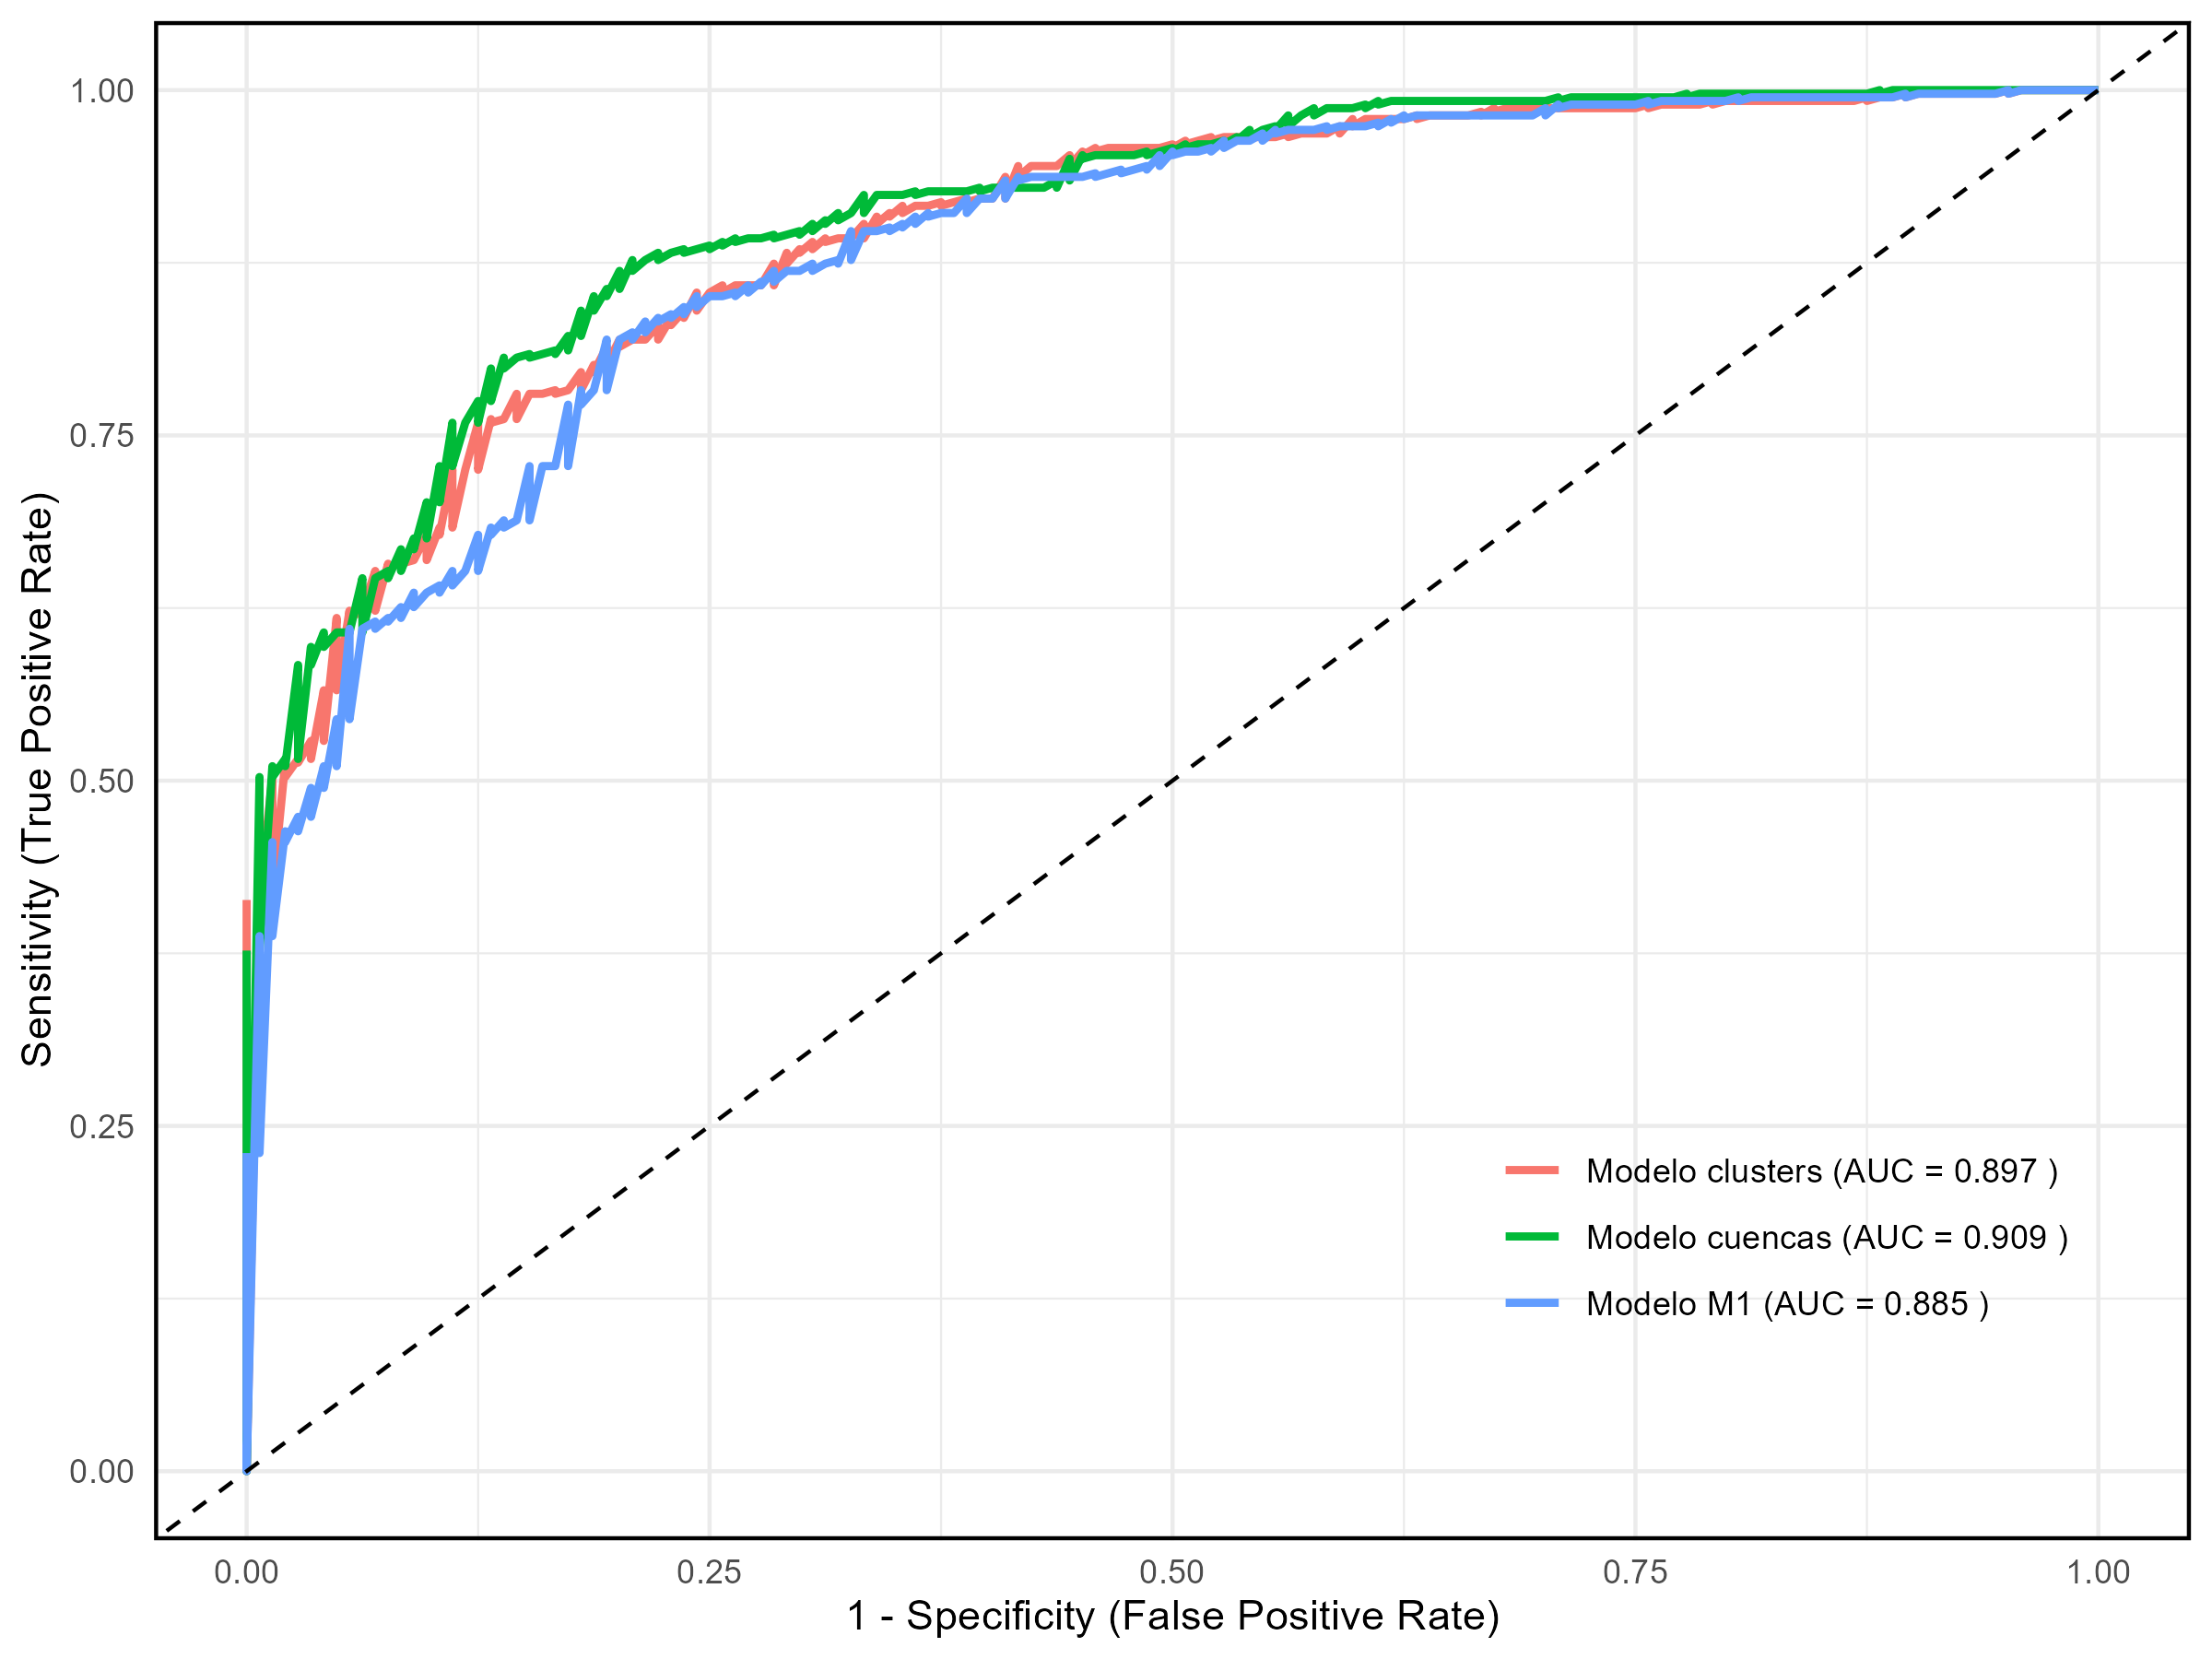
\includegraphics[width=0.8\textwidth]{figures/roc_curve_plot.png}}
\caption{Curvas ROC para los modelos de regresión logística multinivel, mostrando el rendimiento predictivo de cada modelo en términos de sensibilidad frente a 1 - especificidad. Se incluyen los valores del área bajo la curva (AUC) como medida de discriminación del modelo.}
\end{figure}

La Figura \ref{fig:map} presenta la distribución espacial de la susceptibilidad a movimientos en masa dentro del área de estudio, utilizando el modelo de regresión logística multinivel con cuencas como regiones. La zona central del área de estudio muestra predominantemente una alta susceptibilidad, en cuencas con laderas de fuertes pendientes, alto relieve y procesos geomorfológicos activos. Las regiones del este y noroeste presentan una susceptibilidad comparativamente menor. Caracterizada por cuencas con pendientes más suaves y menor elevación.

\begin{figure}[ht!]
    \label{fig:map}
    \centering
      {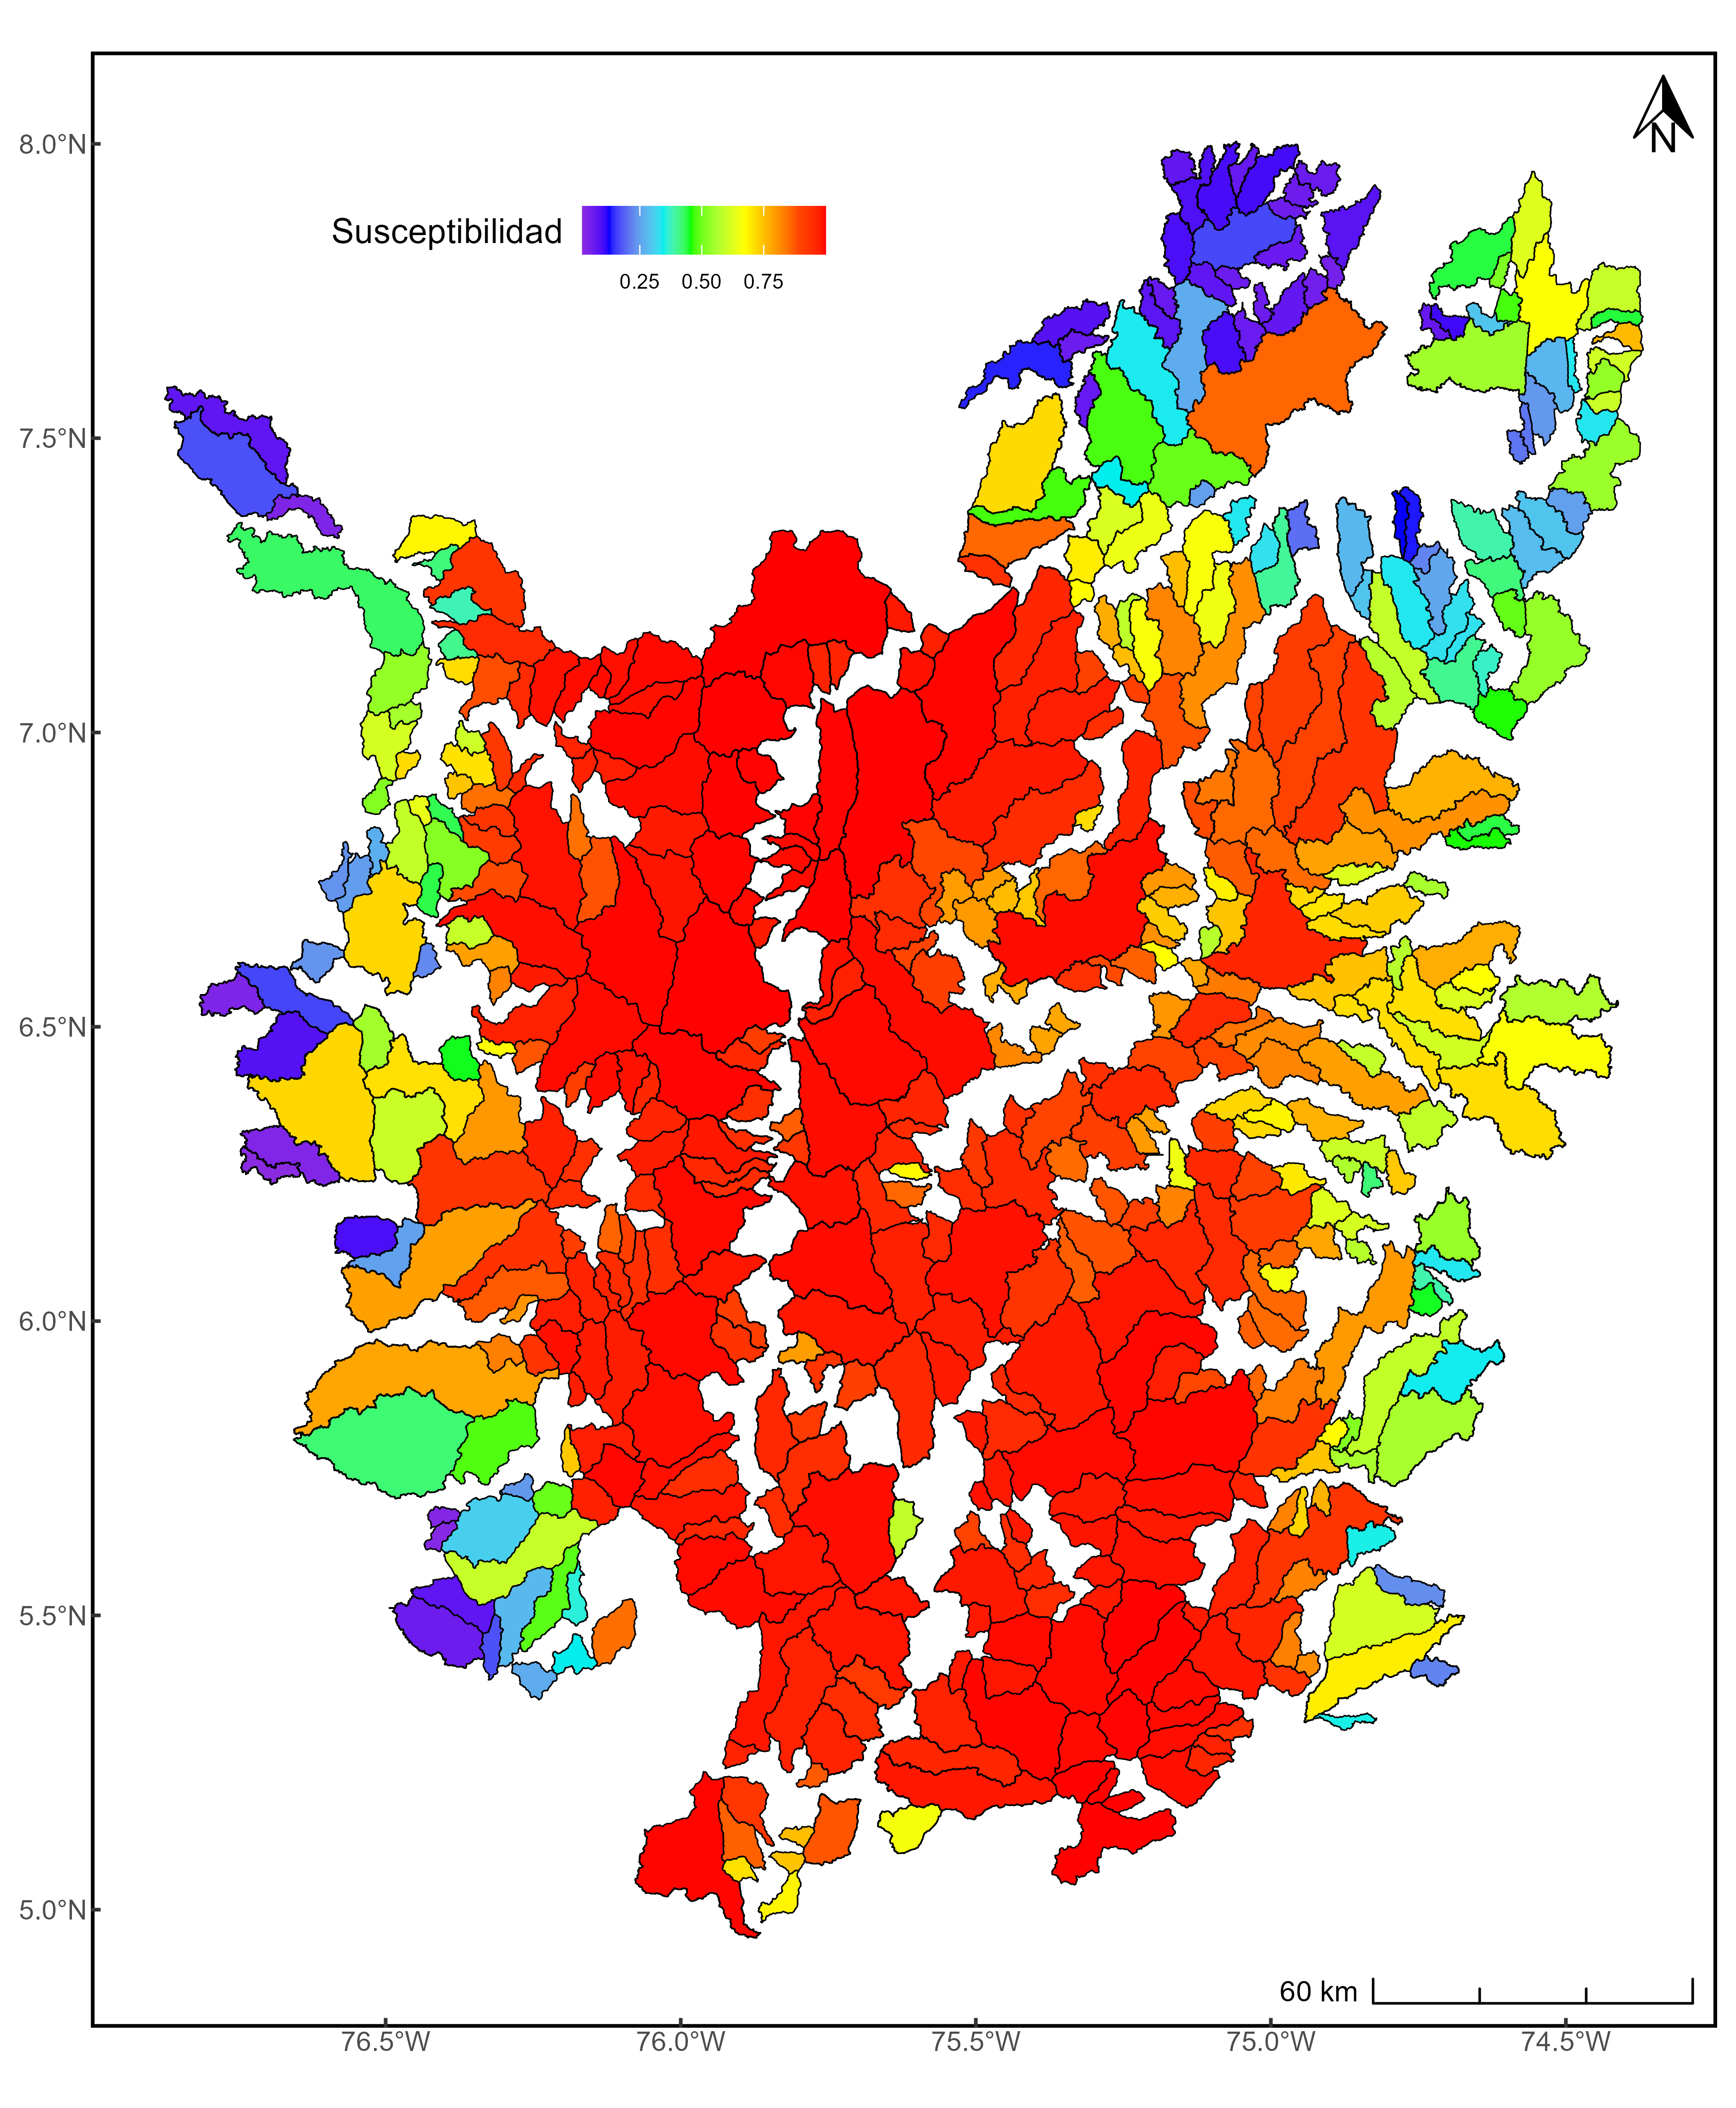
\includegraphics[width=0.8\textwidth]{figures/Mapafinal.png}}
\caption{Distribución espacial de la susceptibilidad a movimientos en masa en el área de estudio utilizando el modelo de regresión logística multinivel agrupada en cuencas hidrográficas. La susceptibilidad se expresa en una escala continua que varía desde baja (azul y verde) hasta muy alta (rojo).}
\end{figure}

\section{Discusión}

La evolución de los modelos de regresión para evaluar la susceptibilidad a movimientos en masa ha avanzado considerablemente, evolucionando de modelos lineales tradicionales a la familia de Modelos Lineales Generalizados (GLM) (\cite{fox2015applied}). Los GLM extienden la capacidad de los modelos lineales al permitir la modificación de la función de enlace, que define cómo se relaciona la media de la variable respuesta como una función de las variables predictoras. En el caso de los modelos de regresión logística esta función de enlace es la función \textit{logit}. Esto facilita la representación de relaciones más complejas entre las variables predictoras y la variable respuesta. Lo cual es esencial para capturar la complejidad de la ocurrencia de movimientos en masa, ya que este fenómeno involucra relaciones no lineales entre factores como la pendiente, la geología, el uso del suelo y las precipitaciones. Además, los GLM permiten la la integración de estructuras jerárquicas, como los modelos multiniveles, lo cual es fundamental para capturar las variaciones espaciales inherentes al problema. 

La incorporación de efectos espaciales y la consideración de la heterogeneidad del terreno son importantes para la evaluación adecuada de la susceptibilidad a movimientos en masa. Suponer que las variables predictivas tienen una influencia homogénea en toda la región puede conducir a interpretaciones erróneas y a generalizaciones que no son adecuadas (\cite{anselin1990spatial, lesage2009introduction}). Por ejemplo, en una región montañosa, la pendiente puede tener una influencia mucho mayor en la ocurrencia de movimientos en masa en comparación con una región plana, donde el uso del suelo o las características del suelo podrían ser factores más determinantes. Ignorar esta heterogeneidad puede llevar a predicciones que no capturan adecuadamente las condiciones locales. Los modelos multiniveles proporcionan una solución robusta para manejar la heterogeneidad del terreno, permitiendo la modelación de la variación de los coeficientes en diferentes unidades espaciales sin incrementar significativamente la complejidad computacional (\cite{wong1985hierarchical}). Estos modelos logran capturar las diferencias espaciales inherentes y permiten evaluar la variabilidad local, lo cual es particularmente relevante en áreas como los Andes colombianos, donde existe una significativa variabilidad geomorfológica y geológica (\cite{aristizabal2015susceptibility}). De esta manera, los modelos multiniveles pueden ofrecer una representación más precisa de los patrones de susceptibilidad a movimientos en masa.

La definición adecuada de las regiones de análisis es un componente esencial en el éxito de los modelos de susceptibilidad a movimientos en masa, ya que una regionalización incorrecta puede resultar en la pérdida de información relevante o en la generación de límites que no reflejan las verdaderas características geomorfológicas y dinámicas de la zona, y llevar a un ajuste deficiente del modelo. En este estudio se exploraron dos enfoques de regionalización: una regionalización natural basada en cuencas y otra basada en un análisis de agrupamiento espacial mediante técnicas de clusterización. Ambos agrupamientos presentan ventajas diferentes. La regionalización natural utiliza cuencas hidrográficas, las cuales representan divisiones geográficas alineadas con procesos geomorfológicos y proporcionan una estructura lógica para el análisis de la dinámica hidrológica y de movimientos en masa. Por otro lado, los grupos definidos mediante agrupamiento espacial permiten crear regiones homogéneas desde un punto de vista morfométrico, en este caso, independientemente de las divisiones hidrológicas del terreno. Los resultados indicaron que la regionalización basada en cuencas presentó un mejor ajuste general, lo cual podría estar vinculado con la coherencia de los límites hidrográficos respecto a la dinámica de los movimientos en masa. No obstante, en futuros trabajos, podrían explorarse otras estrategias de regionalización para determinar si existe una forma de mejorar la capacidad predictiva del modelo.

El uso de unidades de mapeo del terreno apropiadas es fundamental para una evaluación adecuada de la susceptibilidad a movimientos en masa. En este trabajo se utilizaron subcuencas como unidades de mapeo, lo cual permitió una discretización que respeta los patrones naturales a escala regional. La mayoría de los estudios de susceptibilidad emplean celdas regulares en mapas ráster (\cite{arnone2016effect}), lo cual, si bien facilita el análisis y la aplicación de técnicas computacionales, no necesariamente refleja las características naturales del paisaje.  Esta representación arbitraria puede resultar inadecuada para capturar la dinámica de los movimientos en masa, dado que no respeta las divisiones naturales del terreno. En contraposición, estudios recientes han sugerido el uso de unidades de mapeo más representativas del terreno, como subcuencas para estudios regionales o unidades de ladera para estudios locales (\cite{erener2012landslide}), proporcionando una mejor representación de los factores que contribuyen a la inestabilidad del terreno. Estos enfoques permiten una evaluación más precisa de la susceptibilidad y mejoran la capacidad de los modelos para identificar áreas de susceptibilidad o amenaza.

La regresión logística ha sido ampliamente utilizada para la evaluación de la susceptibilidad a movimientos en masa, principalmente debido a su capacidad para modelar la probabilidad de ocurrencia de eventos binarios. Sin embargo, este enfoque presenta limitaciones significativas, particularmente cuando se intenta modelar la ocurrencia de múltiples movimientos en masa en áreas discretas de mayor extensión a celdas regulares ()\cite{lombardo2018point}. La naturaleza binaria de la variable dependiente no permite distinguir entre la ocurrencia de un solo evento o múltiples eventos. es decir en una unidad de mapeo solo se puede especificar la ocurrencia (1) o no ocurrencia de movimientos en masa (0). Cuando se trabaja con celdas que representen el mismo tamaño de los movimientos en masa pueden ser adecuadas. Pero para unidades de mapeo con áreas mayores a los movimientos en masa, cada unidad de mapeo puede tener mas de un movimiento en masa, lo cual no se puede representar en los modelos de regresión logística, y puede resultar en una subestimación o sobrestimación de la susceptibilidad. En contraste, la regresión de tipo Poisson, también perteneciente a la familia de los GLM, ofrece la posibilidad de modelar el número de movimientos en masa esperados, mejorando la interpretación del modelo cuando se trata de áreas donde la frecuencia de movimientos en masa varía (\cite{lombardo2020space}). Este enfoque proporciona una forma más robusta de capturar la naturaleza del fenómeno y de reflejar la dinámica de los movimientos en masa en áreas más complejas.

Un aspecto que requiere una mayor atención en los estudios de susceptibilidad a movimientos en masa utilizando técnicas estadísticas es la evaluación rigurosa del desempeño estadístico de los modelos. En muchos estudios, la evaluación del modelo se limita únicamente a la capacidad predictiva, utilizando herramientas como la curva ROC y el área bajo la curva (AUC). Aunque estas métricas son útiles, no aportan información sobre la validez estadística. Para asegurar la robustez y consistencia de los modelos, es crucial evaluar la significancia estadística de las variables predictoras, la aleatoriedad de los residuos, la ausencia de colinealidad y la homogeneidad de la varianza. La significancia estadística asegura que las variables predictoras contribuyan de manera relevante al modelo; la aleatoriedad de los residuos garantiza que el modelo no esté dejando patrones sin explicar; la ausencia de colinealidad evita problemas de redundancia entre variables predictoras, que podrían sesgar los resultados; y la homogeneidad de la varianza indica que el modelo se comporta de manera consistente a lo largo de toda la muestra. Estas validaciones no solo permiten seleccionar el mejor modelo, sino también asegurar que las relaciones entre las variables predictoras y la variable respuesta sean coherentes y representen adecuadamente el comportamiento del fenómeno.

\section{Conclusiones}
En este estudio se ha implementado un modelo de regresión logística multinivel para evaluar la susceptibilidad a movimientos en masa en los Andes colombianos, utilizando tanto divisiones naturales en cuencas hidrográficas como un enfoque basado en clusterizacion espacial. Los resultados muestran que la consideración de la heterogeneidad espacial y la incorporación de efectos aleatorios mediante modelos multiniveles proporcionan una representación más precisa de la susceptibilidad a movimientos en masa, comparada con los modelos tradicionales de regresión logística que asumen una homogeneidad espacial inadecuada para este tipo de fenómenos.

En el análisis comparativo de los enfoques de regionalización, se observó que la regionalización basada en cuencas hidrográficas logró un mejor ajuste global según las métricas de AIC y BIC, en comparación con el modelo basado en grupos derivados del agrupamiento espacial. Esto sugiere que las divisiones naturales, como las cuencas, al menos en nuestra zona de estudio, proporcionan límites más consistentes para la dinámica de los movimientos en masa, alineados con los procesos geomorfológicos e hidrológicos subyacentes.

En cuanto a la aplicación de modelos multiniveles, este estudio demuestra que la utilización de efectos aleatorios para capturar la heterogeneidad espacial es importante para mejorar la interpretación y la capacidad predictiva de los modelos de susceptibilidad a movimientos en masa. La incorporación de efectos aleatorios no solo permite entender mejor cómo varía la susceptibilidad entre diferentes regiones, sino que también ofrece una representación más robusta de los patrones que influyen en la inestabilidad del terreno. De esta manera, los modelos multiniveles ofrecen una metodología flexible y detallada que puede adaptarse a la naturaleza jerárquica y compleja de los fenómenos geológicos en ambientes montañosos.

\begin{acknowledgement}
El presente trabajo se realizo con el apoyo de la Fundación Alexander von Humboldt (\url{https://www.humboldt-foundation.de/}) a través del programa \textit{Georg Forster Research Fellowship} para investigadores.
\end{acknowledgement}

\section{Open Research}
Data and code used for this study are fully available in Github (\url{https://github.com/edieraristizabal/ModeloMultinivel}).

\printbibliography

\end{document}
